\documentclass{article}
\pdfpagewidth=8.5in
\pdfpageheight=11in


\usepackage{ijcai23}
\usepackage{times}
\usepackage{soul}
\usepackage{url}
\usepackage[hidelinks]{hyperref}
\usepackage[utf8]{inputenc}
\usepackage[small]{caption}
\usepackage{graphicx}
\usepackage{amsmath}
\usepackage{amsthm}
\usepackage{booktabs}
\usepackage{algorithm}
\usepackage{algorithmic}
%\usepackage[switch]{lineno}

\urlstyle{same}

\newtheorem{example}{Example}
\newtheorem{theorem}{Theorem}

\pdfinfo{
/RelatórioFinal
}


\title{Database-driven Chatbot}


% Single author syntax
\author{
    Eduardo Neves
    \affiliations
    Universidade de Coimbra
    \emails
    email@example.com
}


\begin{document}

\maketitle

\begin{abstract}
    No panorama atual vemos em várias plataformas algoritmos de comunicação com pessoas. Entre muitas aplicações, estes podem ser encontrados em vários \textit{websites} banais. A sua utilidade no mundo empresarial viu até crescer mecanismos de construção personalizada de \textit{Chatbots}. Neste trabalho planeia-se desenvoler os mecanismos para a construção de um \textit{Chatbot AI} a partir de \textit{Machine Learning}.
\end{abstract}

\section{Introdução}
A Chatbot is 


\section{Dados e Abordagem}
Os dados para um \textit{Chatbot} baseiam-se principalmente em sequências de interações entre partes. Os \textit{datasets} podem variar entre pergunta e resposta, a e-mails trocados ou conversas em plataformas online entre indivíduos. Para este trabalho foi usado um conjunto de dados baseado em em legendas de filmes para português.

\subsection{Conjunto de dados}
O pacote de dados usado foi tirado do projeto "OPUS ... the open parallel corpus" \cite{opus}, um 'corpus' de testos traduzidos da internet baseada em produtos 'open source'. Este conjunto é atualmente ditribuío pela plataforma "opensubtitles" \cite{opensubtitles}, de onde foi retirado o conteúdo.

Como o foco do projeto é um algoritmo em portguês, retirou-se o dataset "pt", que coleciona mais de 500000 ficheiros de legendas de filmes até o ano de 2017. Separados por anos, alguns filmes contam com várias versões do mesmo filme. O seu tratamento é explicado na secção seguinte. 

\subsection{Tratamento dos dados}
Com o conjunto de dados inicial com redundâncias e pouco estruturado, procurou-se correr um pequena organização à informação. A organização do fluxo de entrada para treino é feita aquando a inicialização do processo.

\subsubsection{Redução de redundâncias}
Como referido, algumas versões do mesmo filme são dispostas e organizadas em conjunto. Ao remover este entrave, pode-se remover uma camada na diretoria e agrupar apenas por ano. Apesar desta diferenciação não ser necessária poderá ser útil em comparações ortográficas ou até numa maior confiança de traduções mais recentes. Para selecionar o ficheiro mais relevante apenas se retirou o ficheiro com menor volume de espaço no disco para 'performance'.

\subsubsection{Alteração do formato}
O \textit{dataset} original continha apenas ficheiros em .xml, com muitos elementos, como tempos e personagens, desnecessárias a este trabalho. Outra especificação sem relevância é a separação por palavras das falas de cada personagem. Simplificou-se então para um formato .json, onde cada entrada é a fala de uma personagem. Manteve-se a separação dos ficheiros por filmes.

\begin{figure}
	\centering
    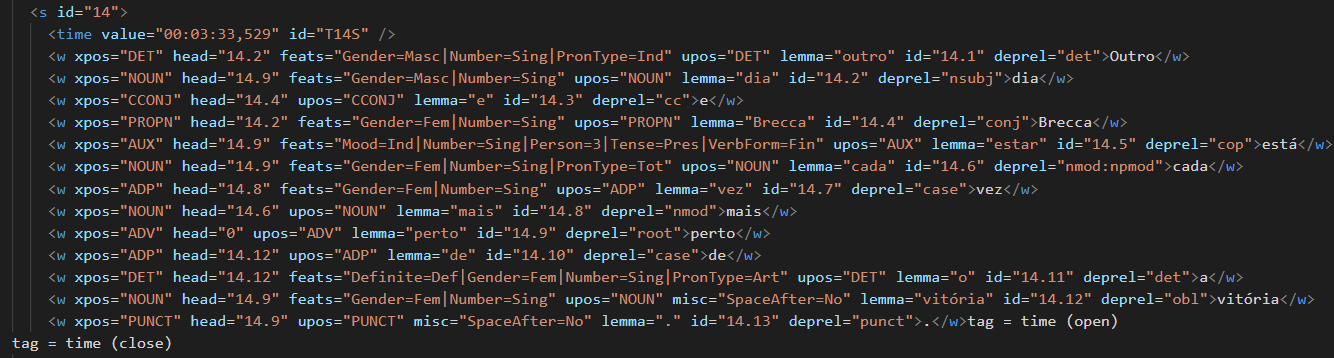
\includegraphics[scale=0.3]{xml.png}
    \caption{Formato original do \textit{dataset} para um filme aleatório}
    \label{xmlimg}
\end{figure}

\begin{figure}
	\centering
    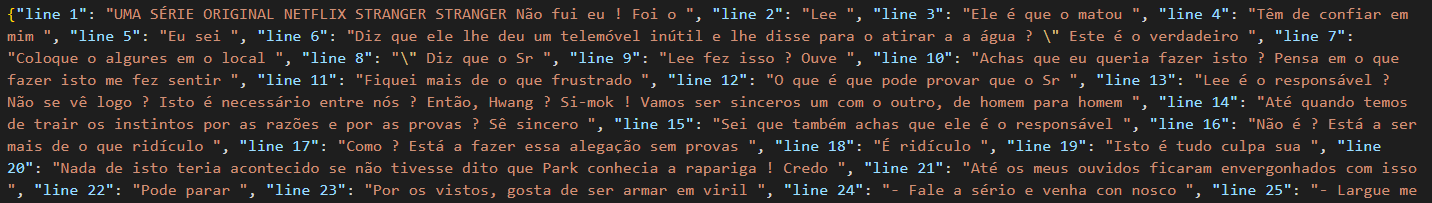
\includegraphics[scale=0.3]{json.png}
    \caption{Formato alterado de um filme aleatório do conjunto}
    \label{jsonimg}
\end{figure}

\subsubsection{Redução de amostragem}
Para além da redução na alteração do formato, reduziu-se também a quantidade de dados usados para o programa. Utilizou-se apenas filmes a partir de 2000, o que resultou em 37851 filmes, com uma média de 455 falas de personagens. Este ainda assim é um número muito grande de filmes, mas manteve-se para manuntenção da utilidade do conjunto, além de uma maior escolha entre filmes de várioa anos para possível teste.

\subsubsection{Preparação para treino}
Na língua portuguesa deparamo-nos com vários acentos e outros símobolos como os traços (como exemplo "ensino-te"). Quanto aos acentos, a sua mantenção é imperativa para boa leitura e para remoção de confusões entre palavras (como por exemplo "estás" e "estas"). Por outro lado, os traços foram retirados, já que a flexão do pronomes quanto ao número e género é demasiado vasta para garantir um vocabulário conciso por parte do modelo. Outros símbolos de síntaxe e gramaticais foram retirados aquando a preparação para treino.


\subsection{Modelo}
O modelo base foi retirado da plataforma Github, do repositório Seq2Seq-Chatbot \cite{abonia2020seq2seq}. Este modelo usa o módulo \textit{tensorflow} para os processos de ML.

No trabalho citado foi também usado um \textit{dataset} de filmes, o 'Cornell Movie Dialog Corpus' \cite{cornell}. Este dispunha de 304713 entradas para treino num ficheiro .txt também disponibilizado.

\subsubsection{LSTM}
A 'Long Short Term Memory' (LSTM) é uma rede neuronal recorrente capaz de aprender a dependência em problemas de predição. Este é útil em tradução, reconhecimento de fala e, direcionado para este tópico, simulação de conversação humana. Mais sobre este tipo de redes, elas têm um estado interno que consegue representar informação em contexto \cite{bengio1994learning}.

\subsubsection{Seq2seq}
A metodologia 'sequence-to-sequence' (seq2seq) é a peça-chave do trabalho. A metodologia utiliza modelos de 'Machine Learning' (ML) para obeter um sequência como entrada, num domínio, e convertê-la para uma representação noutro domínio. 

O \textit{seq2seq} baseia-se num bloco \textit{encoder} que lê a série de entrada a partir de um vetor de dimensionalidade fixa e um bloco \textit{decoder} que extrai a frase. Ambos estes blocos são células LSTM e são treinados ao mesmo tempo \cite{sutskever2014sequence}. Entre eles há um vetor de contexto que encapsula todo o sentido da frase.

\begin{figure}[h]
    \centering
    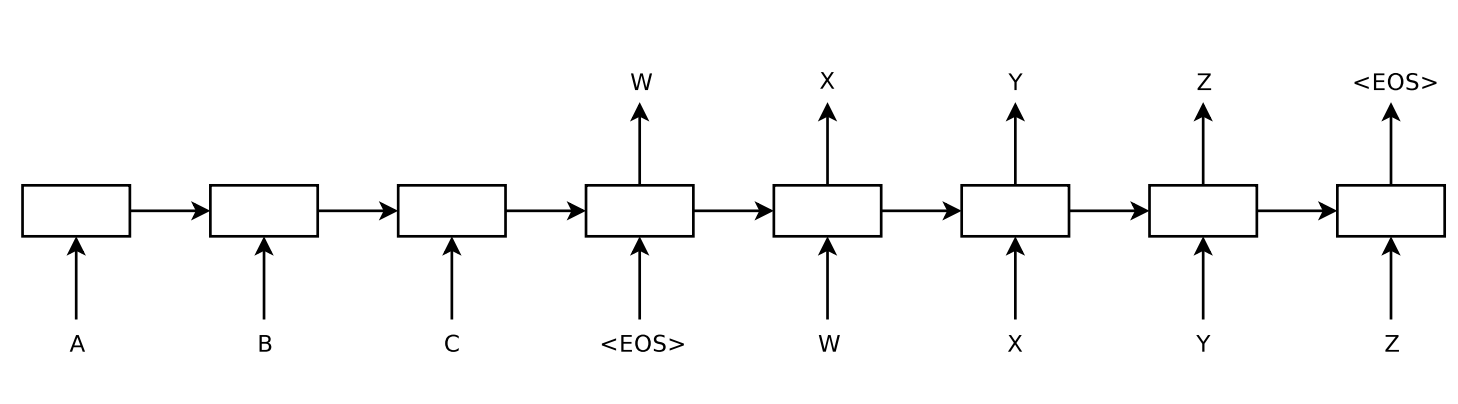
\includegraphics[scale=0.3]{encoder_decoder.png}
    \caption{Ilustração da metodologia. os primeiros quatro retêngulos referem-se à camada \textit{encoder} enquanto o resto pertence à \textit{decoder}}
    \cite{sutskever2014sequence}
    \label{fig1}
\end{figure}


No momento inicial, quando é fornecida uma sequência ao modelo, a frase terá de caber no vetor fixo, portanto leva um \textit{padding}. À sequência acrescenta-se a componente "\textless PAD\textgreater ". Ao passar pelo vetor, o \textit{decoder} inicia com o comando "\textless START\textgreater ", ou "\textless GO\textgreater " como usado neste trabalho, para iniciar a produção da saída. A sequência é completa com a expressão "\textless EOS\textgreater " que simboliza o final do \textit{output}. Para expressões que o algoritmo não reconhece lança-se o comando "\textless UNK\textgreater ".

\subsubsection{'Attention'}
Em ML esta técnica tem o objetivo de reproduzir atenção cognitiva (comportamento humano). o efeito traduz-se em realçar algumas partes da entrada, enquanto diminui outras, mudando o foco da informação dada. Este método é também sensível ao contexto, algo que é tido em conta no treino da máquina. 


\section{Experimentação e Métricas}

\subsection{ROUGE}
'Recall-Oriented Understudy for Gisting Evaluation' é um conjunto de métricas espcializadas em avaliar \textit{machine translation}. Estas métricas focam-se em quanto as palavras (ou \textit{n-grams} no input se assemelham às previstas pelo modelo.

Neste trabalho foca-se no ROUGE-L que se baseia na subsequência mais longa em comum entre o \textit{output} e a referência. Uma vantagem do uso desta métrica é que não é necessário ter correspondências consecutivas, mas correspondências em sequência \cite{rouge}. A implementação é feita com recurso ao módulo "rouge" do \textit{python}.

\section{Resultados}



\section{Problemas e Resoluções}

\subsection{Conjunto de dados}
Alguns problemas foram encontrados no uso da informação.

Em primeiro lugar, muitos ficheiros continham referências aos tradutores como parte das legendas. Como estas variavam em formato e local era difícil prever e retirar estas informações com sucesso.

Algumas traduções eram também desvirtuadas do português Portugal, tais como o uso de expressões como "em a", em vez de "na" em vários locais. A fonte oferecia também um pacote de português Brasil, portanto estas nuances não se esperariam no conjunto usado. Pequenas alterações como esta seriam de difícil execução sem uma análise extensiva dos dados.

\subsubsection{Resolução}


Apesar destes problemas, usou-se este 'dataset' pela sua vastidão e facilidade de acesso. Acrescendo a dificuldade de materiais para a língua desejada, esta foi a melhor opção encontrada.

\subsection{Modelo}
A escolha do código foi influenciada na metodologia seq2seq (aconselhada pelo professor). A pesquisa foi então restringida para tal.

O uso desta versão 1.14 do \textit{tensorflow} é desatualizada, pois o pacote está já na versão 2 a partir de 2019. Esta veio com uma mudança na organização e, portanto, na sintaxe a usar para construir o modelo. Obriga, também, ao uso de uma versão anterior do python (3.6 ou menor). 

Este modelo traz então algumas agravantes, em especial o tempo de compilação. Para 500 filmes com 100 \textit{epochs}, o tempo estimado era de cerca de 13 horas, todo o processo de treino. Com estes números o modelo leva a um esforço computacional aquém do esperado, tornando-se até inexequível em termos de desenvolvimento do trabalho.

Guardar os pesos ocupa muito espaço!!!!?


\section{Conclusions}


\bibliographystyle{named}
\bibliography{biblio.bib}

\end{document}

